

Stability analysis of non-linear differential equations is not an easy task. Many of the methods used for stability analysis require a linear pde. Since the KS-equation is stiff, it is not easy to find a good approximation for the non-linear term, $\frac{1}{2}(u^2)_x$, since it stabilizes the solution. One opportunity is to substitute 

\begin{align*}
\frac{1}{2}(u^2)_x \approx \frac{1}{2}(\rho(x)u)_x
\end{align*} 

such that $\rho(x)$ is not dependent on time. 

Von Neumann stability analysis is a method based on Fourier decomposition of numerical error, and is used to check the stability of linear pde's. 


\subsection*{Stability analysis of implicit scheme}

 
Choosing $\rho(x) = f(x,0) = U^0$, we obtain the linearized scheme where $R$ is the matrix representing $\rho(x)$:


\begin{align*}
\left( I + \frac{k}{2h^2}A + \frac{k}{2h^4}A^2\right) U^{n+1} = \left( I - \frac{k}{2h^2}A - \frac{k}{2h^4}A^2 - \frac{k}{4h} DR \right)U^{n},
\end{align*}
%
%which written out becomes
%
%\begin{align*}
%U^{n+1}_m + \frac{k}{h^2}(U_{m+1}^{n+1}-2U_{m}^{n+1}+U_{m-1}^{n+1}) + \frac{k}{h^4}(U_{m+2}^{n+1}-4U_{m+1}^{n+1}+6U_m^{n+1}-4U_{m-1}^{+1}n+U_{m-2}^{n+1}) \\
% = U^n_m - \frac{k}{h^2}(U_{m+1}^n-2U_{m}^n+U_{m-1}^n)
%- \frac{k}{h^4}(U_{m+2}^n-4U_{m+1}^n+6U_m^n-4U_{m-1}^n+U_{m-2}^n) \\
%- \frac{k}{4h}(U_{m+1}^0 U_{m+1}^n-U_{m-1}^0 U_{m-1}^n) 
%\end{align*}
%
%Let $U_m^n = \xi^n e^{i \beta x_m}$ and $U_{m}^0 = \xi^0 e^{i\beta x_m} = e^{i\beta x_m}$ such that
%
%\begin{align*}
%\xi (1 + \frac{k}{h^2}(e^{i\beta h}-2+e^{-i\beta h}) + \frac{k}{h^4}(e^{2i\beta h}-4e^{i\beta h}+6-4e^{-i\beta h}+e^{-2i\beta h}) \\
% = 1 - \frac{k}{h^2}(e^{i\beta h}-2+e^{-i\beta h}) - \frac{k}{h^4}(e^{2i\beta h}-4e^{i\beta h}+6-4e^{-i\beta h}+e^{-2i\beta h}) \\
% - \frac{k}{4h}(e^{i\beta h}e^{i\beta h} - e^{-i\beta h}e^{-i\beta h})
% \end{align*}
% 
% 
% \begin{align*}
%\xi &= \frac{1-\frac{k}{h^2}(\cos(\beta h)-1) - \frac{k}{2h^4}(6-8\cos(\beta h)+\cos(2\beta h)) - \frac{k}{2h}i\sin(2\beta h)}{1+\frac{k}{h^2}(\cos(\beta h)-1)+\frac{k}{2h^4}(6-8\cos(\beta h)+2\cos(2\beta h))} \\
%&= \frac{1+\frac{2k}{h^2}\sin^2\left(\frac{\beta h}{2}\right)-\frac{8k}{h^4}\sin^4\left(\frac{\beta h}{2}\right)- \frac{k}{2h}\sin^2(2\beta h)}{1 - \frac{2k}{h^2}\sin^2\left(\frac{\beta h}{2}\right) + \frac{8k}{h^4}\sin^4\left(\frac{\beta h}{2}\right)}
%\end{align*}
%
%Let $q = \sin^2(\frac{\beta h}{2})$ and $r = \frac{k}{h^4}$. The Von Neumann's stability criterion claims there is a constant $\mu \ge 0$ such that $|\xi| \le 1+ \mu k$. 
%
%% Norm of \xi squared
%\begin{align*}
%|\xi|^2 &= \left(\frac{1+2rq(h^2-4q)}{1 - 2rq(h^2-4q)}\right)^2 + \frac{1}{4}\frac{krh^2\sin^2(2\beta h)}{\left(1 - 2rq(h^2-4q)\right)^2}
%\end{align*}
%
%Maximizing $-2rq(4q-h^2)$ wrt $q$ gives $q = h^2/8$, which replaced in the equation gives

%\begin{align*}
%|\xi |^2 &\le \left(\frac{1+rh^4/8}{1-rh^4/8}\right)^2 + \frac{1}{4}kh^2r \frac{\sin(2\beta h)}{(1-rh^4/8)^2} \\
%&\le \left(\frac{1+k/8}{1-k/8}\right)^2 + k\frac{rh^2}{4(1-k/8)^2}
%\end{align*}



The Von Neumann's stability criterion claims there is a constant $\mu \ge 0$ such that $|\xi| \le 1+ \mu k$ where $\mu$ is independent on both $h$ and $k$. This is not the case in our analysis, as 

\begin{align*}
|\xi |^2 \le \left(\frac{1+k/8}{1-k/8}\right)^2 + k\frac{rh^2}{4(1-k/8)^2},
\end{align*}

so the method is not stable. This is expected, since the linearized KS-equation is unstable in numerical experiments. 

Using an averaging over time, $\rho(x) = (U^{N_0}-U^0)/2$, where $U^{N_0}$ represents the solution after $N_0$ iterations, we observed a solution slightly more similar to the solution from the non-linear scheme, but also here we observed a non-stability.
 
Numerically, it seems that stability for the implicit scheme only is dependent on $k$. This hypothesis is strengthened by the fact that when $h$ tends to zero, the bound for $k$ converges from below to $k \approx 1/3$.

%%%%%%%%%%%%%%%%%%%%%%%%%%%%%%%%%%%%%%%%%%%%%%%%%%%%%

\subsection*{Stability analysis of explicit scheme}

The explicit scheme is stable when $k < r \cdot h^4$. Let us now use Von Neumann stability analysis on the explicit scheme with the same $\rho(x) = U^0$:


\begin{align*}
U^{n+1} = \left(I - \frac{k}{h^2}A - \frac{k}{h^4}A^2 - \frac{k}{4h} DR\right)U^{n} 
\end{align*}


\begin{align*}
\xi = 1 - \frac{k}{h^2}(e^{i\beta h}-2+e^{-i\beta h}) - \frac{k}{h^4}(e^{2i\beta h}-4e^{i\beta h}+6-4e^{-i\beta h}+e^{-2i\beta h}) \\
 - \frac{k}{4h}(e^{i\beta h}e^{i\beta h} - e^{-i\beta h}e^{-i\beta h})\\
\end{align*}

Let $r = k/h^4$ as before.

\begin{align*}
|\xi |^2 &= (1-4rh^2(\cos(\beta h)-1)-2r(3-4\cos(\beta h)+\cos(2\beta h)))^2 + k\frac{rh^2}{4}\sin^2(2\beta h) \\
&= \left(1+4rh^2\sin^2\left(\frac{\beta h}{2}\right)-16r\sin^4\left(\frac{\beta h}{2}\right)\right)^2 + k\left(\frac{rh^2}{4}\sin^2(2\beta h)\right)
\end{align*}

We want $|\xi| \le 1+ \mu k$, so we need 
\begin{align*}
\psi = |1+4rh^2\sin^2\left(\frac{\beta h}{2}\right)-16r\sin^4\left(\frac{\beta h}{2}\right)| \le 1 + \tilde{\mu}k.
\end{align*}
Let $q = \sin^2\left(\frac{\beta h}{2}\right)$ and assume that $(1 \le 16rq^2 \le 2)$ and $(0 \le 4rh^2q \le 1)$


\begin{align*}
\psi = \left| 1+4rh^2q -16rq^2\right| \le \left| 1-16rq^2\right| \le 1 \underset{0\le q\le 1}{\implies} \left(1/16 \le r \le 1/8 \right)
\end{align*} 

\begin{align*}
|\xi |^2 &\le |1-16rq^2|^2 + k\frac{rh^2}{4} = |16rq^2-1|^2  + k\frac{rh^2}{4} \\
\textrm{Inserting } r = 1/8: \\
&\le |16\frac{1}{8}q^2-1|^2 + k\frac{h^2}{8\cdot 4} = |2q^2-1| + k\frac{h^2}{32} \\
&\le 1 + k\frac{h^2}{32}
\end{align*}

Under the assumptions above, we have not shown stability, since $\mu$ is $h$-dependent. This is not surprising, since the linear solution is unstable in experiments, as shown in figure \ref{fig:lin_exp}. Still, the upper bound for $r$ is an interesting result, as it corresponds to the experimental bound for the explicit scheme. For approximately $k/h^4 \le 1/8$ the explicit scheme provides a stable solution. 




\begin{figure}[H]
\centering
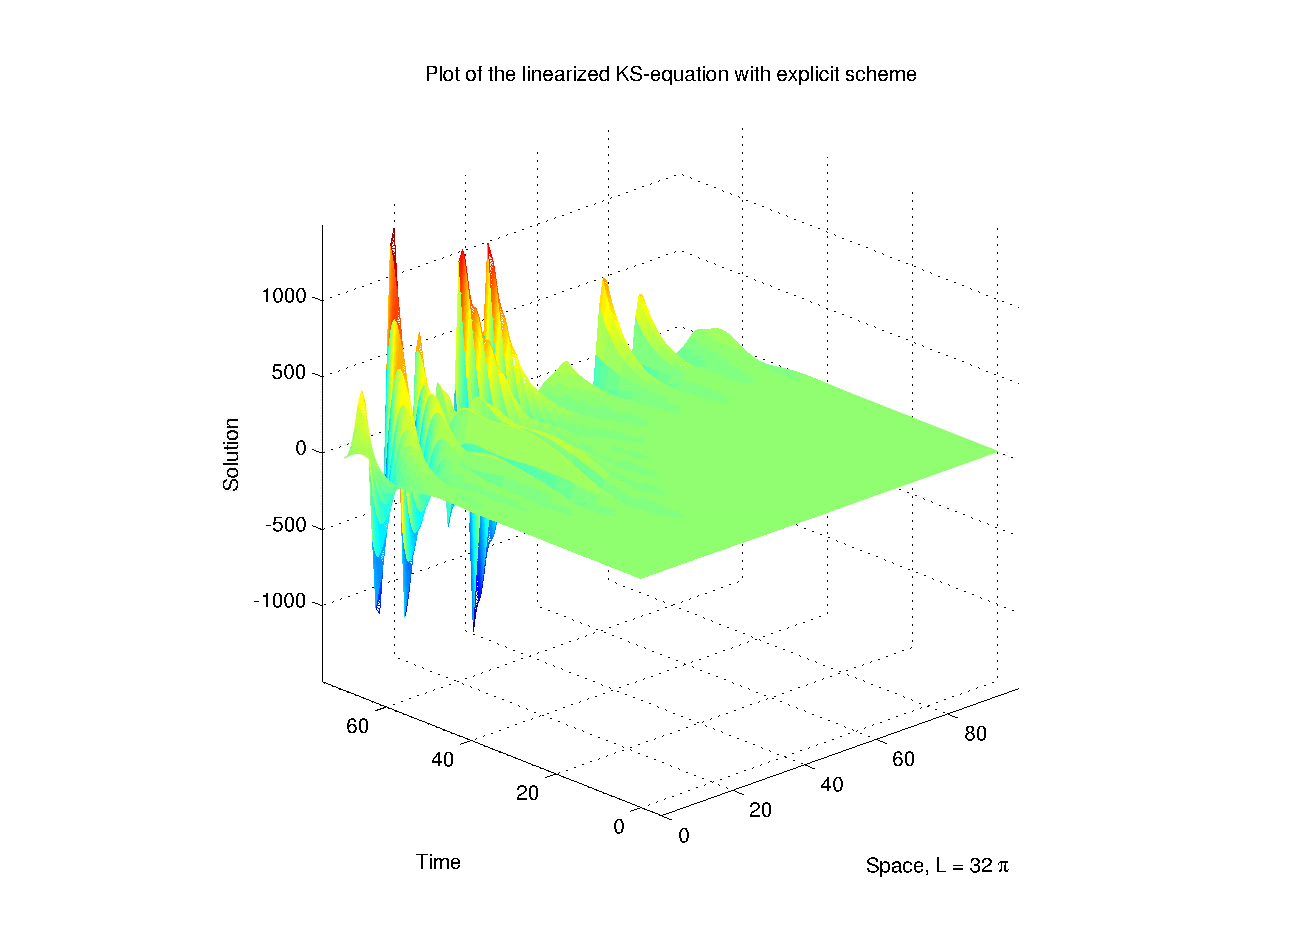
\includegraphics[scale=0.5]
{../PDFs/FE_Exp/linear_explicit.pdf}
\caption{Surface plot of $u(x,t)$ on the linearized explicit scheme. The method is unstable for all $r$.}
\label{fig:lin_exp}
\end{figure}







